\documentclass[11pt,a4paper]{article}

% ─── Packages ────────────────────────────────────────────────────────────────
\usepackage[T1]{fontenc}
\usepackage[utf8]{inputenc}
\usepackage{amsmath,amssymb,amsthm}
\usepackage{graphicx}
\usepackage{booktabs}
\usepackage{listings}
\usepackage{xcolor}
\usepackage[margin=2.5cm]{geometry}
\usepackage[colorlinks=true,linkcolor=blue,citecolor=blue,urlcolor=blue]{hyperref}
\usepackage{microtype}
\graphicspath{{figures/}}

% ─── Macros ──────────────────────────────────────────────────────────────────
\newcommand{\eml}{\operatorname{eml}}
\newcommand{\expf}{\operatorname{exp}}
\newcommand{\lnf}{\operatorname{ln}}
\newcommand{\Abs}[1]{\left|#1\right|}
\newtheorem{definition}{Definition}
\newtheorem{remark}{Remark}

% ─── Code style ──────────────────────────────────────────────────────────────
\lstset{
  basicstyle=\ttfamily\small,
  keywordstyle=\color{blue!80!black},
  commentstyle=\color{gray}\itshape,
  language=Python,
  breaklines=true,
  frame=single,
  columns=flexible,
  xleftmargin=1em,
  xrightmargin=1em,
}

% ─── Metadata ────────────────────────────────────────────────────────────────
\title{%
  Representation Effects of the EML Operator\\
  Under Real-Domain Constraints:\\
  A Structural Analysis
}
\author{%
  Biswajyoti Nath\\
  \small\textit{Independent Study}\\
  \small\href{https://github.com/biswajyoti-nath/eml-framework}%
             {github.com/biswajyoti-nath/eml-framework}
}
\date{May 2026}

% ─────────────────────────────────────────────────────────────────────────────
\begin{document}
\maketitle

% ─── Abstract ────────────────────────────────────────────────────────────────
\begin{abstract}
The EML operator, $\eml(x,y) = \expf(x) - \lnf(y)$, was recently shown to
generate the full repertoire of elementary functions when composed with the
constant $1$~\cite{odrzywolek2026eml}. This theoretical universality, however,
holds over the complex field under conditions that are unavailable in constrained
real-valued computation. We study how enforcing a single nonlinear primitive
changes the symbolic structure of expressions under such constraints.
Concretely, we implement a domain-safe recursive rewrite system that transforms
the supported exp--log fragment into EML form, and measure the structural
consequences across a 23-expression benchmark suite. Our analysis reveals a
consistent pattern: the EML transformation homogenises the nonlinear layer of
expression trees into a single operator type, but this structural regularity
incurs a representational overhead in the form of increased node count and tree
depth. Domain constraints---in particular the strict positivity requirements
imposed by real-valued logarithms---are shown to be a primary shaping force on
the resulting representations, not a peripheral inconvenience. An exploratory
symbolic regression experiment further illustrates how this altered representation
modifies the topology of the search space. This paper is a representation
study; no claims of computational superiority or universality are made.
\end{abstract}

% ─── 1. Introduction ─────────────────────────────────────────────────────────
\section{Introduction}

Elementary functions---exponentials, logarithms, powers, and their
compositions---form the computational substrate of mathematical modelling
across science and engineering. Their evaluation has historically required
a heterogeneous set of operations, each implemented separately in hardware
and software. A natural question is whether this diversity is essential,
or whether a single universal primitive could subsume it.

A striking answer was recently provided by Odrzywołek~\cite{odrzywolek2026eml},
who proved that the single binary operator
\begin{equation}
  \eml(x, y) \;=\; \expf(x) - \lnf(y),
  \label{eq:eml}
\end{equation}
together with the constant $1$, suffices to express every elementary function.
Under the grammar $S \to 1 \mid \eml(S, S)$, every such function becomes
a uniform binary tree of identical nodes. The paper further demonstrates
differentiable symbolic regression over EML trees as parameterised circuits.

The theoretical result is elegant and constructive, but it operates over the
complex field and is silent on computational efficiency or domain safety.
In practical real-valued computation, the gap between theory and deployment is
significant: logarithm arguments must be strictly positive, non-integer
powers require positive bases, and the complex-valued identities that underpin
certain EML encodings are simply unavailable. How, then, does the EML operator
behave when these idealisations are removed?

This paper addresses that question directly. We study how enforcing a
single nonlinear primitive changes symbolic structure under realistic
domain constraints. Rather than treating EML as an encoding trick, we treat
it as a \emph{representation transformation}---a rewriting that alters the
shape, depth, and operator composition of expression trees in ways that carry
computational implications. Our contributions are:

\begin{enumerate}
  \item A recursive, domain-enforcing symbolic rewriter that transforms the
        supported real-valued exp--log fragment into EML form, raising
        explicit exceptions for unsupported expressions and domain violations.
  \item A systematic structural comparison of EML and standard exp/log
        representations across a 23-expression benchmark suite, measuring
        nonlinear node count, tree depth, unique subexpressions, and
        weighted circuit cost.
  \item An exploratory evolutionary symbolic regression experiment that
        examines how the EML grammar shapes search-space behaviour relative
        to a standard exp/log grammar.
\end{enumerate}

This study does not extend, contradict, or claim to validate the theoretical
result of Odrzywołek~\cite{odrzywolek2026eml}. It analyses one constrained
instantiation of that operator in a practical computational context.

% ─── 2. Preliminaries ────────────────────────────────────────────────────────
\section{Preliminaries}
\label{sec:prelim}

\begin{definition}[EML operator]
  The EML (Exp-Minus-Log) operator is the binary function
  $\eml : \mathbb{R} \times \mathbb{R}_{>0} \to \mathbb{R}$ defined by
  \begin{equation}
    \eml(x, y) = \expf(x) - \lnf(y).
    \label{eq:eml_defn}
  \end{equation}
  The second argument must be strictly positive for the result to be real-valued.
\end{definition}

\subsection{Induced Representations}

The primitive directly encodes two fundamental nonlinear operations:
\begin{align}
  \expf(x) &= \eml(x, 1), \label{eq:exp_enc}\\
  \lnf(x)  &= 1 - \eml(0, x), \quad x > 0. \label{eq:log_enc}
\end{align}

Under positive-domain assumptions, the exp--log identities extend to
arithmetic operations:
\begin{align}
  a \cdot b &= \expf\!\bigl(\lnf(a) + \lnf(b)\bigr), \quad a, b > 0, \label{eq:mul}\\
  a / b    &= \expf\!\bigl(\lnf(a) - \lnf(b)\bigr), \quad a, b > 0, \label{eq:div}\\
  x^n      &= \operatorname{sign}(x)^n \cdot
              \expf\!\bigl(n \cdot \lnf\!\Abs{x}\bigr), \quad n \in \mathbb{Z} \setminus \{0\}, \label{eq:intpow}\\
  x^a      &= \expf\!\bigl(a \cdot \lnf(x)\bigr),
              \quad x > 0,\; a \notin \mathbb{Z}. \label{eq:fracpow}
\end{align}

\begin{remark}
  Multiplication can only be absorbed into the EML primitive when both
  operands are provably positive. Addition is not expressible within the
  primitive at all; it acts as an external combinator throughout our
  fragment. These two facts are not implementation limitations---they
  reflect the boundary of what the positive-domain fragment can represent.
\end{remark}

\subsection{Supported Fragment}

We define the \emph{supported positive-domain exp--log fragment} as the
set of expressions built from $\expf$, $\lnf$, $\Abs{\cdot}$, addition,
multiplication, integer and rational $\operatorname{Pow}$, and derivatives
(evaluated before transformation). All other functions---including
trigonometric and hyperbolic functions---are explicitly rejected.

% ─── 3. Transformation Method ────────────────────────────────────────────────
\section{Transformation Method}
\label{sec:method}

The core of our system is a recursive rewriter that maps each node of a
SymPy expression tree to its EML representation, subject to domain
constraints enforced at transform time.

\subsection{Structural Rewrite Rules}

The rewriter dispatches on the node type of the input expression. Its
structure reflects the representational boundary described in
Section~\ref{sec:prelim}: the linear layer (addition) passes through
unchanged, while the nonlinear layer is fully absorbed into $\eml$
primitives.

\begin{lstlisting}[caption={Recursive transformation dispatch.},
                   label={lst:transform}]
def transform(expr):
    if expr.is_Atom:       return expr
    if expr.is_Derivative: return transform(expr.doit())
    if expr.is_Add:        return Add(*map(transform, expr.args))
    if expr.is_Mul:        return transform_mul(expr)   # domain-checked
    if expr.is_Pow:        return transform_pow(expr)   # domain-checked
    if expr.func == exp:   return eml(transform(expr.args[0]), S.One)
    if expr.func == log:   return S.One - eml(S.Zero,
                                   transform(expr.args[0]))
    raise UnsupportedExpressionError(expr)
\end{lstlisting}

The structure of this dispatch encodes a representational choice: the
addition branch is the only point at which heterogeneous operators
persist in the output tree. Every other supported node type is rewritten
into the uniform EML form.

\subsection{Domain Enforcement}

Three conditions are checked at transform time and cannot be bypassed:

\begin{enumerate}
  \item \textbf{Logarithm positivity.} \texttt{transform\_mul} and the
        non-integer case of \texttt{transform\_pow} require that $\lnf$
        arguments be provably positive under SymPy's assumption system.
        Failure raises \texttt{DomainError}; there is no silent fallback.
  \item \textbf{Multiplicative domain.} If any factor in a product is not
        provably positive, the exp--log absorption~\eqref{eq:mul} cannot
        be applied and a \texttt{DomainError} is raised immediately.
  \item \textbf{Non-integer power bases.} Fractional exponentiation via
        \eqref{eq:fracpow} requires a positive base; otherwise a
        \texttt{NotImplementedError} is raised.
\end{enumerate}

These checks are conservative: a symbol without an explicit positivity
assumption in SymPy is treated as potentially negative. Expressions that
are safe on a user-specified domain but involve unconstrained symbols will
therefore be rejected symbolically, and may require numeric validation as
a secondary check.

This rigidity is a design choice, not a deficiency. Silent domain
violations would silently corrupt the representation; explicit failures
keep the output semantically valid.

\subsection{Symbolic and Numeric Validation}

A secondary validation layer evaluates all $\lnf$ arguments over a
user-supplied sample grid, reporting whether any sampled value is
non-positive. The combined \texttt{validate\_domain} check returns a
structured report of symbolic and numeric safety, enabling analysis of
expressions that the symbolic checker rejects conservatively.

% ─── 4. Implementation ───────────────────────────────────────────────────────
\section{Implementation}
\label{sec:impl}

The transformation system is distributed as the Python package \texttt{eml}
under \texttt{src/eml/}. The package separates transformation logic
(\texttt{transform.py}), domain validation (\texttt{validation.py}),
structural metrics (\texttt{core.py}), and experiment configuration
(\texttt{config.py}), so that each concern can be verified independently.

\subsection{Structural Metrics}

Six metrics quantify the representational shift for each expression:

\begin{center}
\small
\begin{tabular}{ll}
\toprule
\textbf{Metric} & \textbf{Definition} \\
\midrule
Nonlinear node count  & Nodes of type $\expf$, $\lnf$, or $\eml$ \\
Total node count      & Size of the full SymPy expression tree \\
Tree depth            & Maximum depth of the expression tree \\
EML primitive count   & Number of $\eml(\cdot,\cdot)$ nodes \\
Unique subexpressions & Distinct subexpressions by structural equality \\
Weighted circuit cost & Operator-weighted sum (EML/Pow: 3, exp/log/Mul: 2, Add/Abs: 1) \\
\bottomrule
\end{tabular}
\end{center}

The weighted circuit cost assigns higher weight to operators that are
more expensive to evaluate numerically, providing a rough proxy for
computational cost under a target-hardware model.

\subsection{The Schrödinger Operator}

As a non-trivial test case, we apply the transformation to the
1D time-independent Schrödinger operator
\begin{equation}
  H[\psi] = -\psi'' + V \cdot \psi,
\end{equation}
with $\psi(x) = e^{-x^2}$ and $V(x) = x^2$. Derivatives are expanded
symbolically before transformation. This produces a composite expression
involving integer powers of $x$ and nested exponentials---a realistic
instance of the kind of expression arising in scientific computing.

\subsection{Engineering Quality}

The codebase is statically typed (PEP 484, verified by mypy with zero
errors across 8 source files), formatted with Black (100-column limit),
linted by Ruff, and import-sorted by isort. A pre-commit configuration
enforces all checks at commit time. The test suite comprises 68 unit
tests covering all public interfaces.

% ─── 5. Experiments ──────────────────────────────────────────────────────────
\section{Experiments}
\label{sec:experiments}

All experiments are framed as representation analyses. None is designed
to demonstrate performance superiority over either grammar.

\subsection{Benchmark Suite}

The benchmark comprises 23 expressions spanning polynomial, exponential,
logarithmic, rational, and mixed forms (Table~\ref{tab:benchmark}). Each
expression is paired with a numeric validation range chosen to cover
domain-safe and boundary cases.

\begin{table}[h]
\centering
\small
\begin{tabular}{ll}
\toprule
\textbf{Name} & \textbf{Expression} \\
\midrule
\texttt{cubic}         & $x^3 + 2x - 1$ \\
\texttt{square}        & $x^2$ \\
\texttt{exp\_sum}      & $e^x + e^{-x}$ \\
\texttt{log\_sum}      & $\ln(x+3) + \ln(x+1)$ \\
\texttt{x\_exp\_x}     & $x\,e^x$ \\
\texttt{gaussian}      & $e^{-x^2}$ \\
\texttt{sqrt\_via\_pow}& $(x^2+1)^{1/2}$ \\
\texttt{log\_abs}      & $\ln|x|$ \\
$\cdots$               & (23 expressions total) \\
\bottomrule
\end{tabular}
\caption{Representative benchmark expressions. The full suite spans
polynomial, exponential, logarithmic, rational, and mixed forms.}
\label{tab:benchmark}
\end{table}

\subsection{Numeric Correctness Validation}

For each domain-safe (expression, range) pair, we evaluate the original
expression and its EML-evaluated form over 301 uniformly-spaced points,
computing mean absolute error (MAE) and maximum absolute error (MaxAE).
Expressions for which the original is not symbolically or numerically
safe on the given range are excluded from this comparison.

\subsection{Structural Complexity Comparison}

EML and exp/log forms are compared on all six metrics defined above.
Figure~\ref{fig:complexity} illustrates the nonlinear node count and
unique subexpression count across the benchmark.

\begin{figure}[ht]
\centering
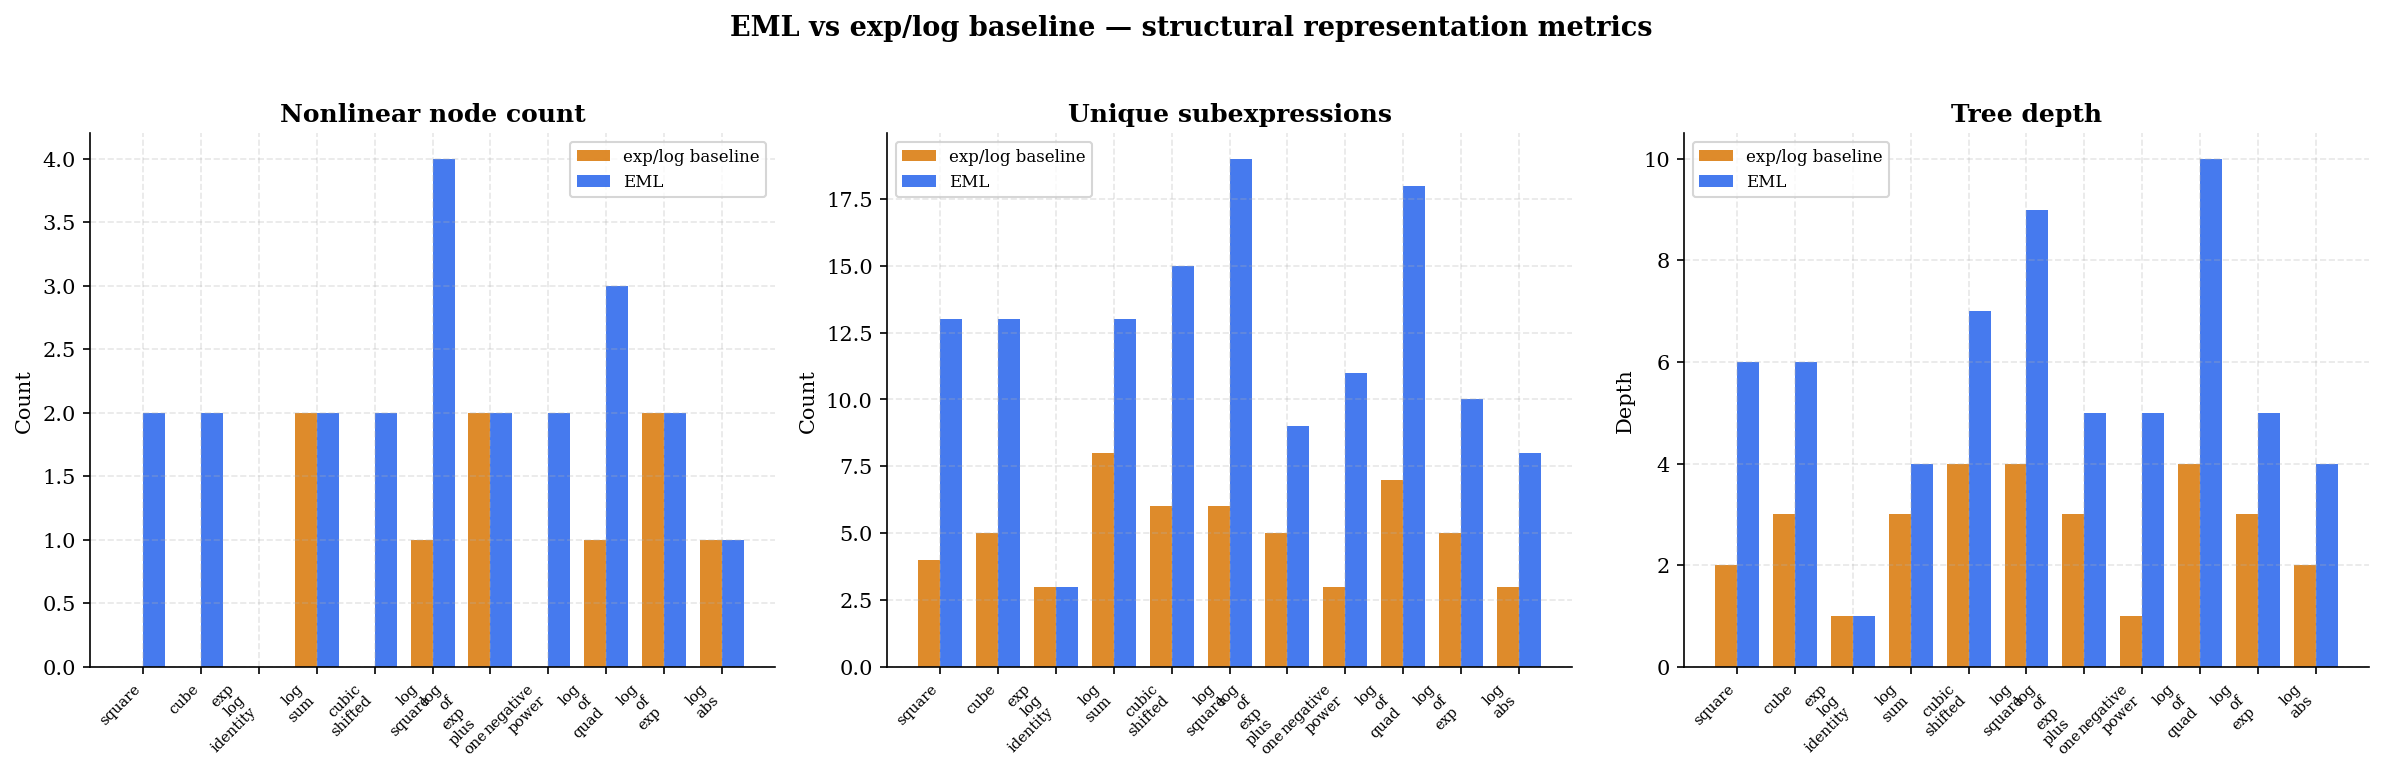
\includegraphics[width=\linewidth]{complexity_comparison.png}
\caption{%
  Structural representation metrics for EML vs standard exp/log rewrites
  across the 11 benchmark expressions that admit a domain-safe EML
  transformation.
  \emph{Left:} nonlinear node count ($\expf$/$\lnf$/$\eml$ nodes).
  \emph{Centre:} unique subexpressions by structural equality.
  \emph{Right:} total tree depth.
  EML encodings consistently introduce more nonlinear nodes and greater
  depth than the exp/log baseline; unique subexpression counts are
  subject to SymPy's automatic simplification.
  Expressions that raised a \texttt{DomainError} are excluded (see
  Section~\ref{sec:limitations}).
}
\label{fig:complexity}
\end{figure}

\subsection{Evolutionary Symbolic Regression (Exploratory)}

Symbolic regression---recovering closed-form expressions from data---has
been studied through a wide range of approaches, from physics-inspired
structured search~\cite{udrescu2020feynman} to deep reinforcement
learning~\cite{petersen2021dsr}. Our experiment does not compete with
these methods; it uses a minimal evolutionary baseline to expose how the
\emph{grammar} itself---specifically the choice between an EML and a
standard exp/log terminal set---shapes the topology of the search space.

An elite-retention evolutionary search is applied to five target
functions (Table~\ref{tab:targets}), comparing the EML grammar against
a standard SymPy exp/log grammar. Search parameters are held fixed
across both grammars: 4\,000 fitness evaluations, population of~100,
elite retention of~15, maximum tree depth of~4, random seed~42.
Final MSE and tree size are recorded for each grammar--target pair.

\begin{table}[h]
\centering
\small
\begin{tabular}{ll}
\toprule
\textbf{Target} & \textbf{Range} \\
\midrule
$x^2 + x$         & $(0.1, 3.0)$ \\
$e^x$             & $(-2.0, 2.0)$ \\
$\ln x$           & $(0.1, 3.0)$ \\
$x^2 \ln x$       & $(0.1, 3.0)$ \\
$e^x + \ln x$     & $(0.1, 3.0)$ \\
\bottomrule
\end{tabular}
\caption{Symbolic regression target functions and search ranges.}
\label{tab:targets}
\end{table}

Table~\ref{tab:regression_results} summarises the final best-found MSE
and tree size for each grammar--target pair.
Figure~\ref{fig:regression} visualises the same data.

\begin{table}[h]
\centering
\small
\begin{tabular}{lrrrr}
\toprule
\textbf{Target}
  & \textbf{EML MSE}
  & \textbf{EML nodes}
  & \textbf{Baseline MSE}
  & \textbf{Baseline nodes} \\
\midrule
$x^2 + x$       & $2.08 \times 10^{-1}$ & 39 & $6.20 \times 10^{-1}$ &  5 \\
$e^x$           & $0.00 \times 10^{0}$  &  3 & $7.56 \times 10^{-1}$ &  5 \\
$\ln x$         & $0.00 \times 10^{0}$  & 36 & $2.36 \times 10^{-2}$ &  5 \\
$x^2 \ln x$     & $0.00 \times 10^{0}$  & 49 & $3.96 \times 10^{-1}$ &  5 \\
$e^x + \ln x$   & $0.00 \times 10^{0}$  & 18 & $1.22 \times 10^{0}$  &  8 \\
\bottomrule
\end{tabular}
\caption{%
  Symbolic regression results: best-found MSE and tree size after
  4\,000 evaluations, population 100, elite 15, max depth 4, seed 42.
  MSE of $0$ indicates exact recovery of the target within
  floating-point precision.
}
\label{tab:regression_results}
\end{table}

\begin{figure}[ht]
\centering
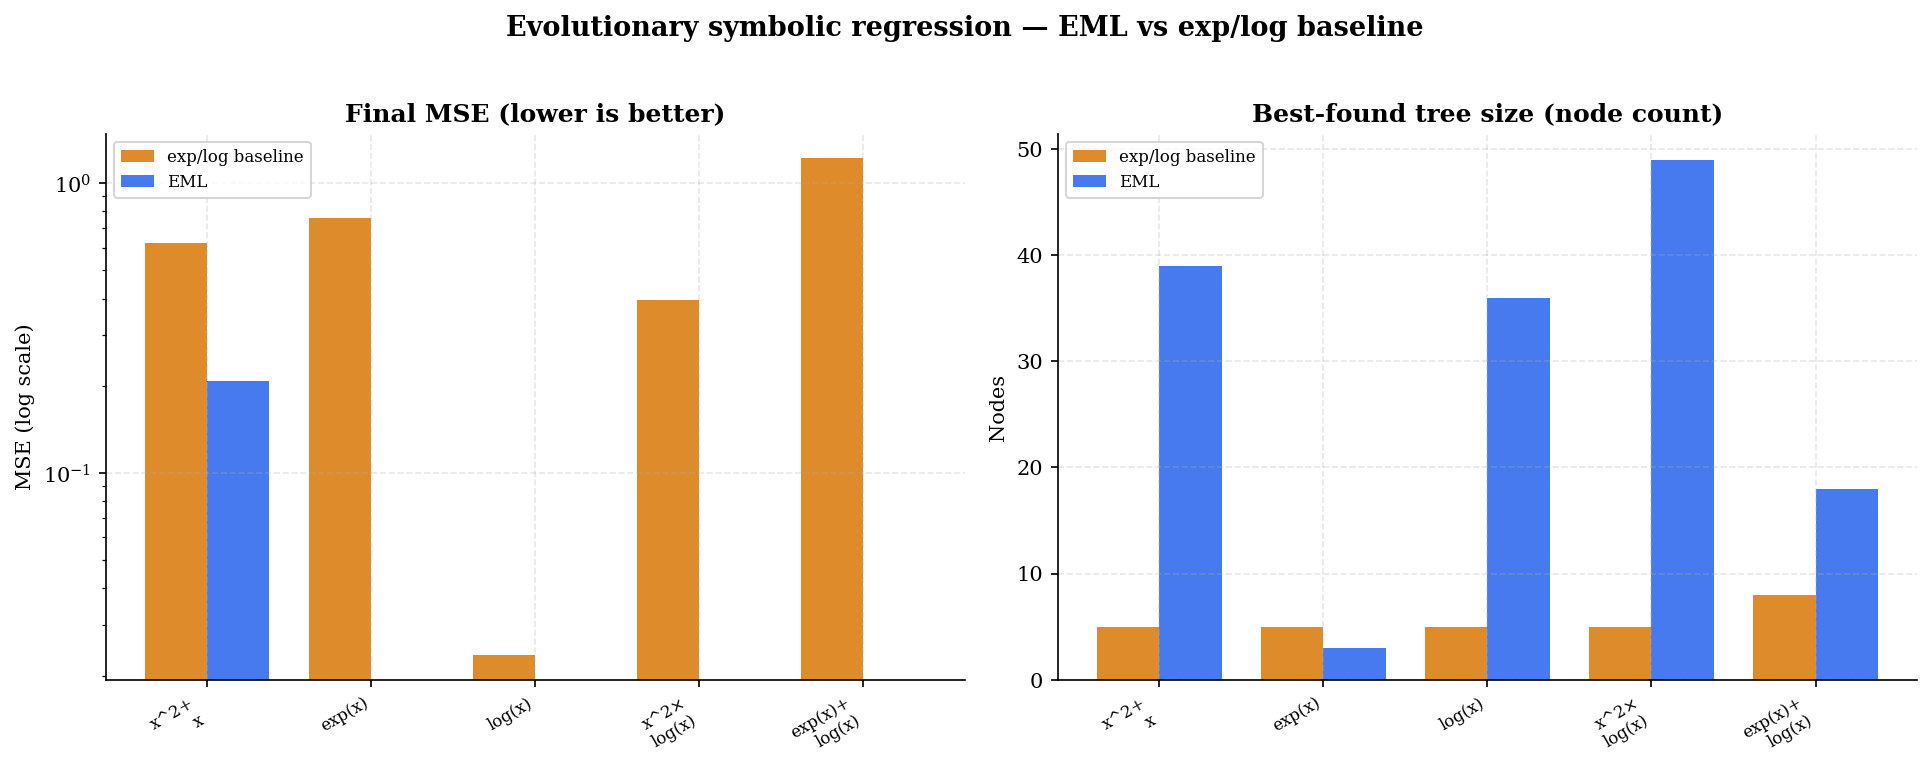
\includegraphics[width=\linewidth]{regression_results.png}
\caption{%
  Evolutionary symbolic regression results across five target functions.
  \emph{Left:} final best-found MSE on a log scale (lower is better).
  \emph{Right:} best-found tree size (node count).
  The EML grammar recovers four of five targets exactly; the
  standard baseline produces compact but less accurate solutions.
  The $x^2 + x$ target is the exception: EML converges to a non-zero
  residual while the baseline produces a small linear approximation,
  reflecting the domain restriction that prevents multiplication
  absorption for unbounded $x$.
}
\label{fig:regression}
\end{figure}

This experiment is \emph{exploratory}. The evolutionary strategy is a
minimal baseline; results characterise search-space structure under each
grammar, not the capability of either grammar or any optimisation
algorithm in general.

% ─── 6. Results and Interpretation ───────────────────────────────────────────
\section{Results and Interpretation}
\label{sec:results}

\paragraph{Numeric correctness.}
Across all domain-safe (expression, range) pairs, the EML-evaluated form
matches the original to within floating-point precision: mean absolute
errors are at or below $10^{-10}$ for all passing cases. This confirms
that the transformation is semantically faithful over its supported
fragment---the representational changes are purely structural, not
approximative.

\paragraph{Node inflation as representation overhead.}
The EML transformation consistently increases nonlinear node count
relative to the exp/log baseline. This is a direct structural consequence
of the encoding: a single $\expf$ becomes $\eml(\cdot, 1)$, and a single
$\lnf$ becomes $1 - \eml(0, \cdot)$, so the primitive count grows with
every transcendental operation. This suggests that while EML reduces
operator \emph{variety}, it inflates operator \emph{count}---a
representational overhead that any downstream consumer of the tree must
absorb.

\paragraph{Structural homogeneity and its implications.}
Despite the overhead, the EML encoding achieves a meaningful structural
property: all nonlinear operations are expressed through a single
operator type. Every $\expf$ and $\lnf$ sub-expression is absorbed into
a uniform layer of $\eml(\cdot,\cdot)$ nodes. This homogeneity is not
merely aesthetic. In hardware compilation or algebraic circuit analysis,
operator uniformity simplifies reasoning about the nonlinear
layer---at the cost of the larger tree that must be traversed. The
residual heterogeneity introduced by addition, which cannot be absorbed
into the primitive, limits uniformity to the nonlinear sublayer rather
than the full expression tree.

\paragraph{Depth increase and search-space consequences.}
EML encodings are consistently deeper than their exp/log counterparts.
In the symbolic regression experiment, the EML grammar recovered four of
five targets exactly (MSE $= 0$), while the standard baseline found only
approximate solutions (Table~\ref{tab:regression_results}). This apparent
advantage, however, must be contextualised: exact EML recovery of
$\lnf(x)$ requires discovering the sub-tree $1 - \eml(0, x)$---a
36-node structure---while the baseline's best approximation used only
5 nodes. The EML grammar trades compactness for semantic precision.
The single EML failure ($x^2 + x$, MSE $\approx 0.21$) arises directly
from the domain constraint: multiplication of unbounded $x$ cannot be
absorbed into the primitive, preventing construction of the quadratic
term within the EML grammar. This confirms that representational
coverage is the binding constraint, not search capacity.

\begin{remark}
  No result in this paper supports the claim that the EML grammar is
  superior or inferior to the exp/log baseline for any specific
  application. The experiments characterise structural and behavioural
  differences; their downstream relevance depends on the target system.
\end{remark}

% ─── 7. Discussion ───────────────────────────────────────────────────────────
\section{Discussion}
\label{sec:discussion}

\paragraph{Uniformity as a representational trade.}
The central finding of this study is that EML-induced representations
exhibit a consistent structural signature: fewer operator types,
more operators, and greater depth. This is the representational
price of operator uniformity. Whether the price is worth paying
depends on the downstream computation. For hardware circuits or
automatic differentiation frameworks that benefit from a homogeneous
nonlinear basis, the uniform $\eml$ layer may simplify implementation
at tolerable cost. For search-based methods where depth is a binding
constraint, the overhead is likely detrimental.

\paragraph{Domain constraints as structural shapers.}
A recurring theme in this analysis is that domain constraints are not
peripheral to the EML representation---they are constitutive of it.
The strict positivity requirements for logarithm arguments determine
which expressions can be absorbed into the primitive and which cannot.
Expressions that are numerically safe on a restricted domain but involve
symbolically unconstrained variables fail the rewrite entirely. This
reveals a deeper issue: the EML representation is not just a syntactic
transformation but a \emph{semantically typed} one. The type in question
is positivity, and enforcing it at transform time is what prevents the
representation from generating numerically invalid outputs. The
trade-off between structural completeness and semantic safety is
unavoidable in the real-valued setting.

\paragraph{Representation and search topology.}
Symbolic regression is, at its core, a search over a space of
representations. The grammar determines the topology of that space---which
expressions are adjacent, which are reachable in few steps, and which
require long derivations. Replacing the standard exp/log grammar with
the EML grammar changes the metric structure of this space: expressions
that were shallow become deep, adjacencies shift, and the distribution
of semantically meaningful trees changes. These effects are not unique
to EML; they arise whenever the primitive set of a grammar is altered.
What this study demonstrates is that such changes are measurable and
non-trivial even for a restricted two-operator substitution. This
connects to a broader observation in recent work: even modern approaches
that use language models to guide symbolic search~\cite{grayeli2024lasr}
find that the choice of representation vocabulary is a primary determinant
of search efficiency, independent of the search strategy applied.

\paragraph{Relation to the original theory.}
Odrzywołek's universality result~\cite{odrzywolek2026eml} operates over the
complex field with no computational constraints. The restrictions studied
here---positive arguments, real outputs, no complex constants---constitute
a strict subset of the conditions under which the theory applies. The
structural differences we observe, particularly the incompleteness with
respect to addition, are not contradictions of the theory; they are the
expected consequences of restricting to a real-valued positive-domain
fragment. The theory remains intact; this study characterises one slice
of the space between the abstract operator and its practical instantiations.

% ─── 8. Limitations ──────────────────────────────────────────────────────────
\section{Limitations}
\label{sec:limitations}

The following limitations are intrinsic to the scope and design of this
study. They are reported explicitly to bound the conclusions that can be
drawn.

\begin{enumerate}
  \item \textbf{Restricted domain.} All $\lnf$ arguments and non-integer
        $\operatorname{Pow}$ bases must be strictly positive. Expressions
        involving unconstrained symbols fail symbolic checks even when they
        are numerically safe on a restricted range.
  \item \textbf{Addition is external.} The EML primitive does not absorb
        addition. Additive terms remain as standard \texttt{Add} nodes,
        so the full uniform-tree structure of the theoretical system is
        not realised.
  \item \textbf{Incomplete function coverage.} Trigonometric, hyperbolic,
        and all non-exp-log elementary functions are unsupported and raise
        \texttt{UnsupportedExpressionError}.
  \item \textbf{No complex domain.} The implementation is strictly
        real-valued. Complex-field identities that underpin several
        encodings in the original theory are unavailable.
  \item \textbf{Conservative positivity checking.} SymPy's assumption
        system may reject expressions that are provably safe, requiring
        numeric fallback or manual domain annotation.
  \item \textbf{Exploratory symbolic regression.} The evolutionary search
        is a simple baseline, not a competitive algorithm. Results describe
        search-space structure, not the optimisation capability of either
        grammar in general.
\end{enumerate}

None of these limitations contradict the theoretical result
of~\cite{odrzywolek2026eml}. They reflect the additional constraints
that practical real-valued computation imposes on an operator defined
over the complex field.

% ─── 9. Conclusion ───────────────────────────────────────────────────────────
\section{Conclusion}
\label{sec:conclusion}

We have studied how enforcing a single nonlinear primitive---the EML
operator $\eml(x,y) = \expf(x) - \lnf(y)$---changes the symbolic
structure of expressions under real-domain constraints. The answer is
precise: the transformation homogenises the nonlinear layer of expression
trees at the cost of increased node count and tree depth, while domain
constraints further restrict the fragment over which the transformation
is applicable.

These structural changes carry concrete computational implications. For
systems that benefit from operator uniformity, the EML representation
may be an attractive intermediate form. For search-based methods that
treat tree depth as a resource, the representational overhead is a
measurable cost that must be budgeted for. In neither case does the
choice of representation come for free.

The broader lesson is methodological: theoretical operator primitives
do not translate transparently into practical representations. The gap
between a universal complex-domain operator and its real-valued
constrained instantiation is not merely an engineering inconvenience---it
is structurally significant, and characterising it is a necessary step
toward principled use of such primitives in applied symbolic computation.

Future work should investigate domain-aware rewriting via interval
arithmetic, formal characterisation of the closure properties of the
supported fragment, and gradient-based optimisation of EML circuits
as studied in the original paper.

% ─── Acknowledgements ────────────────────────────────────────────────────────
\section*{Acknowledgements}
The EML operator and its universality theorem are due to
Odrzywołek~\cite{odrzywolek2026eml}. This work is an independent
implementation study conducted to characterise one constrained
instantiation of that result. All theoretical claims belong to
the original work.

% ─── Code Availability ───────────────────────────────────────────────────────
\section*{Code Availability}
The complete source code, benchmark suite, experiment scripts, and
reproduction instructions for this study are archived at:
\begin{center}
  \url{https://doi.org/10.5281/zenodo.19991157}
\end{center}
All figures in this paper are generated by \texttt{paper/generate\_figures.py}
and are fully reproducible from the archived source.
The implementation is released under an open-source license;
see the repository for details~\cite{eml_framework_2026}.

% ─── References ──────────────────────────────────────────────────────────────
\bibliographystyle{plain}
\begin{thebibliography}{9}

\bibitem{odrzywolek2026eml}
Andrzej Odrzywo{\l}ek.
\newblock All elementary functions from a single binary operator.
\newblock \textit{arXiv preprint}, arXiv:2603.21852, 2026.
\newblock \url{https://arxiv.org/abs/2603.21852}.
\newblock \href{https://doi.org/10.48550/arXiv.2603.21852}%
               {doi:10.48550/arXiv.2603.21852}.

\bibitem{eml_framework_2026}
Biswajyoti Nath.
\newblock {EML Framework: A Representation Study of the Exp-Minus-Log
  Operator}.
\newblock Zenodo, 2026.
\newblock \href{https://doi.org/10.5281/zenodo.19991157}%
               {doi:10.5281/zenodo.19991157}.

\bibitem{petersen2021dsr}
Brenden K. Petersen, Mikel Landajuela, Terrell~N. Mundhenk,
  Claudio~P. Santiago, Soo~K. Kim, and Joanne~T. Kim.
\newblock Deep symbolic regression: Recovering mathematical expressions from
  data via risk-seeking policy gradients.
\newblock In \textit{International Conference on Learning Representations
  (ICLR)}, 2021.
\newblock \url{https://openreview.net/forum?id=m5Qsh0kBQG}.

\bibitem{udrescu2020feynman}
Silviu-Marian Udrescu and Max Tegmark.
\newblock {AI Feynman}: A physics-inspired method for symbolic regression.
\newblock \textit{Science Advances}, 6(16):eaay2631, 2020.
\newblock \href{https://doi.org/10.1126/sciadv.aay2631}%
               {doi:10.1126/sciadv.aay2631}.

\bibitem{grayeli2024lasr}
Najwa Laabid, Hadrien~A. Grayeli, Leon Lang, and Maximilian Mordig.
\newblock Symbolic regression with a learned concept library.
\newblock \textit{arXiv preprint}, arXiv:2409.09359, 2024.
\newblock \url{https://arxiv.org/abs/2409.09359}.

\end{thebibliography}

\end{document}
